\documentclass[a4paper,11pt]{article}
\usepackage{amsmath,amsthm,amsfonts,amssymb,amscd,amstext,vmargin,graphics,graphicx,tabularx,multicol} 
\usepackage[francais]{babel}
\usepackage[utf8]{inputenc}  
\usepackage[T1]{fontenc} 
\usepackage{pstricks-add,tikz,tkz-tab,variations}
\usepackage[autolanguage,np]{numprint} 
\usepackage{calc}

\setmarginsrb{1.5cm}{0.5cm}{1cm}{0.5cm}{0cm}{0cm}{0cm}{0cm} %Gauche, haut, droite, haut
\newcounter{numexo}
\newcommand{\exo}[1]{\stepcounter{numexo}\noindent{\bf Exercice~\thenumexo} : }
\reversemarginpar

\newcommand{\bmul}[1]{\begin{multicols}{#1}}
\newcommand{\emul}{\end{multicols}}

\newcounter{enumtabi}
\newcounter{enumtaba}
\newcommand{\q}{\stepcounter{enumtabi} \theenumtabi.  }
\newcommand{\qa}{\stepcounter{enumtaba} (\alph{enumtaba}) }
\newcommand{\initq}{\setcounter{enumtabi}{0}}
\newcommand{\initqa}{\setcounter{enumtaba}{0}}

\newcommand{\be}{\begin{enumerate}}
\newcommand{\ee}{\end{enumerate}}
\newcommand{\bi}{\begin{itemize}}
\newcommand{\ei}{\end{itemize}}
\newcommand{\bp}{\begin{pspicture*}}
\newcommand{\ep}{\end{pspicture*}}
\newcommand{\bt}{\begin{tabular}}
\newcommand{\et}{\end{tabular}}
\renewcommand{\tabularxcolumn}[1]{>{\centering}m{#1}} %(colonne m{} centrée, au lieu de p par défault) 
\newcommand{\tnl}{\tabularnewline}

\newcommand{\trait}{\noindent \rule{\linewidth}{0.2mm}}
\newcommand{\hs}[1]{\hspace{#1}}
\newcommand{\vs}[1]{\vspace{#1}}

\newcommand{\N}{\mathbb{N}}
\newcommand{\Z}{\mathbb{Z}}
\newcommand{\R}{\mathbb{R}}
\newcommand{\C}{\mathbb{C}}
\newcommand{\Dcal}{\mathcal{D}}
\newcommand{\Ccal}{\mathcal{C}}
\newcommand{\mc}{\mathcal}

\newcommand{\vect}[1]{\overrightarrow{#1}}
\newcommand{\ds}{\displaystyle}
\newcommand{\eq}{\quad \Leftrightarrow \quad}
\newcommand{\vecti}{\vec{\imath}}
\newcommand{\vectj}{\vec{\jmath}}
\newcommand{\Oij}{(O;\vec{\imath}, \vec{\jmath})}
\newcommand{\OIJ}{(O;I,J)}


\newcommand{\reponse}[1][1]{%
\multido{}{#1}{\makebox[\linewidth]{\rule[0pt]{0pt}{20pt}\dotfill}
}}

\newcommand{\titre}[5] 
% #1: titre #2: haut gauche #3: bas gauche #4: haut droite #5: bas droite
{
\noindent #2 \hfill #4 \\
#3 \hfill #5

\vspace{-1.6cm}

\begin{center}\rule{6cm}{0.5mm}\end{center}
\vspace{0.2cm}
\begin{center}{\large{\textbf{#1}}}\end{center}
\begin{center}\rule{6cm}{0.5mm}\end{center}
}



\begin{document}
\pagestyle{empty}
\titre{Séance d'AP 5 : Résoudre des problèmes avec le calcul littéral}{}{}{3ème}{}

\vspace*{0.4cm}

\textit{Vous rendrez sur une feuille simple, 5 des 7 exercices suivants bien rédigés.\\}



\bmul{2}

\exo \\

Prouver que si on choisit le même nombre de départ, on obtient le même résultat final avec ses deux programmes.\\

\includegraphics[scale=1]{apcalcullitt1.eps} 

\columnbreak

\exo \\

Les figures ci dessous ont-elles le même périmètre ? Une démonstration est attendue.\\

\includegraphics[scale=0.4]{apcalcullitt2.eps} 


\emul

\vspace*{0.5cm}




\bmul{2}

\exo \\

\bmul{2}
$x$ désigne un nombre positif. Voici un rectangle dont les côtés sont des longueurs variables.

\columnbreak


\includegraphics[scale=1]{apcalcullitt4.eps} \\

\emul

\bmul{2}
\initq \q Léa a construit le programme suivant avec le logiciel Scratch.\\
 Que représentent les variables $l$ et $L$ ?\\
 
\columnbreak


\includegraphics[scale=0.8]{apcalcullitt3.eps} \\

\emul



\noindent \q Tester ce programme en donnant à $x$ la valeur 3, puis la valeur 10.\\
\q Quel est le rôle du programme de Léa ?\\
\q Léa affirme : "$P =3x+9$ et $A = x^{2} + 7x +10$". A-t-elle raison ? Expliquer votre raisonnement.\\


	
\columnbreak

\exo \\

Marc affirme : " La somme de cinq entiers consécutifs est égale au quintuple du troisième." \\

Marc a-t-il raison ? Justifier votre réponse en démontrant son propos ou en trouvant un contre-exemple.\\

\vspace*{1cm}

\exo \\

Démontrer que les égalités suivantes sont vraies pour n'importe quelles valeurs de $a$ et de $b$.\\

\noindent \initq \q $(a+b)^{2} + (a-b)^{2} = 2(a^{2} + b^{2})$\\
\q $4ab = (a+b)^{2} - (a-b)^{2}$\\
\q $(a+b)(a-b) + b^{2} = ab + a(a-b)$\\

\emul




\bmul{2}

\exo \\

\initq
\q \qa Développer $(x-1)^{2}$.\\
\qa Justifier que $99^{2} = 9 801$ en utilisant le développement précédent.\\

\q \initqa \qa Développer $(x-1)(x+1)$.\\
\qa Justifier que $99 \times 101  = 9 999$ en utilisant le développement précédent.\\




\columnbreak


\exo \\

Aujourd'hui Paul a 11 ans et Pierre  a 26 ans. \\
Dans combien d'année, l'âge de Pierre sera-t-il le double de celui de Paul ? Justifier en détaillant votre raisonnement.\\

\emul







\end{document}
